\documentclass{article}
\usepackage{spconf}

\usepackage{cite}
\usepackage{amsmath,amssymb,amsfonts}
\usepackage{algorithmic}
\usepackage{graphicx}
\usepackage{textcomp}
\usepackage{bm}
\usepackage{upgreek}

\usepackage{hyperref}

\usepackage[retainorgcmds]{IEEEtrantools}



\graphicspath{{../Figures/}}


\DeclareMathOperator*{\argmin}{arg\,min}
\DeclareMathOperator*{\argmax}{arg\,max}

\DeclareMathOperator{\xrm}{\mathrm{x}}
\DeclareMathOperator{\Xrm}{\mathrm{X}}
\DeclareMathOperator{\yrm}{\mathrm{y}}
\DeclareMathOperator{\Yrm}{\mathrm{Y}}
\DeclareMathOperator{\Drm}{\mathrm{D}}
\DeclareMathOperator{\nrm}{\mathrm{n}}
\DeclareMathOperator{\nbarrm}{\bar{\mathrm{n}}}
\DeclareMathOperator{\zrm}{\mathrm{z}}

\DeclareMathOperator{\Prm}{\mathrm{P}}
\DeclareMathOperator{\prm}{\mathrm{p}}
\DeclareMathOperator{\Erm}{\mathrm{E}}
\DeclareMathOperator{\Crm}{\mathrm{C}}
\DeclareMathOperator{\drm}{\mathrm{d}}

\DeclareMathOperator{\Xcal}{\mathcal{X}}
\DeclareMathOperator{\Ycal}{\mathcal{Y}}
\DeclareMathOperator{\Dcal}{\mathcal{D}}
\DeclareMathOperator{\Ncal}{\mathcal{N}}
\DeclareMathOperator{\Zcal}{\mathcal{Z}}
\DeclareMathOperator{\Hcal}{\mathcal{H}}
\DeclareMathOperator{\Fcal}{\mathcal{F}}
\DeclareMathOperator{\Rcal}{\mathcal{R}}
\DeclareMathOperator{\Mcal}{\mathcal{M}}
\DeclareMathOperator{\Scal}{\mathcal{S}}
\DeclareMathOperator{\Pcal}{\mathcal{P}}
\DeclareMathOperator{\Lcal}{\mathcal{L}}

\DeclareMathOperator{\Rbb}{\mathbb{R}}
\DeclareMathOperator{\Rbbgeq}{\mathbb{R}_{\geq 0}}
\DeclareMathOperator{\Nbb}{\mathbb{N}}
\DeclareMathOperator{\Zbb}{\mathbb{Z}}
\DeclareMathOperator{\Zbbgeq}{\mathbb{Z}_{\geq 0}}

\DeclareMathOperator{\Dir}{\mathrm{Dir}}
\DeclareMathOperator{\DM}{\mathrm{DM}}
\DeclareMathOperator{\Multi}{\mathrm{Multi}}
\DeclareMathOperator{\Bi}{\mathrm{Bi}}
\DeclareMathOperator{\DP}{\mathrm{DP}}
\DeclareMathOperator{\DMP}{\mathrm{DMP}}
\DeclareMathOperator{\Emp}{\mathrm{Emp}}
\DeclareMathOperator{\DE}{\mathrm{DE}}
\DeclareMathOperator{\EP}{\mathrm{EP}}
\DeclareMathOperator{\DEP}{\mathrm{DEP}}

\DeclareMathOperator{\thetam}{\theta_\text{m}}
\DeclareMathOperator{\upthetam}{\uptheta_\text{m}}
\DeclareMathOperator{\thetac}{\theta_\text{c}}
\DeclareMathOperator{\upthetac}{\uptheta_\text{c}}

\DeclareMathOperator{\psim}{\psi_\text{m}}
\DeclareMathOperator{\Psim}{\Psi_\text{m}}
\DeclareMathOperator{\uppsim}{\uppsi_\text{m}}
\DeclareMathOperator{\Uppsim}{\Uppsi_\text{m}}
\DeclareMathOperator{\psic}{\psi_\text{c}}
\DeclareMathOperator{\Psic}{\Psi_\text{c}}
\DeclareMathOperator{\uppsic}{\uppsi_\text{c}}
\DeclareMathOperator{\Uppsic}{\Uppsi_\text{c}}

\DeclareMathOperator{\alpham}{\alpha_\text{m}}
\DeclareMathOperator{\alphac}{\alpha_\text{c}}


\interdisplaylinepenalty=2500


\title{Bayesian Learning for Regression using Dirichlet Prior Probability Distributions of Varying Localization}


%\name{Anonymous\thanks{Anonymous.}}
%\address{Anonymous}

\twoauthors
  {Paul Rademacher}
	{U.S. Naval Research Laboratory\\Radar Division\\Washington, DC 20375, USA\\paul.rademacher@nrl.navy.mil}
  {Milo\v{s} Doroslova\v{c}ki}
	{The George Washington University\\Department of Electrical and Computer Engineering\\Washington, DC 20052, USA\\
   doroslov@gwu.edu}





\begin{document}

\maketitle


\begin{abstract}
When taking a Bayesian approach to machine learning applications, the performance of the learned function strongly depends on how well the prior distribution selected by the designer matches the true data-generating distribution. Dirichlet priors have a number of desirable properties - they lead to closed-form posterior distributions given independent training data, have full support over the space of data probability distributions, and can be maximally informative or non-informative depending on their localization parameter. This paper assumes a Dirichlet prior and produces predictive distributions to characterize unobservable random quantities given observed data. The results are then applied to the most common loss function for regression, the squared-error loss. The optimal Bayes estimator and the resultant risk trends are presented for different prior localizations, demonstrating a bias/variance trade-off.
\end{abstract}

\begin{keywords}
Bayesian learning, machine learning, regression, estimation, Dirichlet distribution, predictive distribution
\end{keywords}



\section{Introduction}

The success or failure of Bayesian learning methods hinge on how well the prior knowledge imparted by the designer matches reality. The chosen prior distribution over the set of data-generating probability distributions reflects the users confidence that different distributions are responsible for generating the observed/unobserved random elements. If a highly localized prior is chosen that strongly weights the actual data probability distribution, low risk learning functions are possible even with limited training data; however, if the localized prior is poorly selected, a good solution may not be achieved. Conversely, a non-informative prior that effects fast adaptation during training; if data is limited, however, the learning function may not deliver the required performance.

This work assumes that the joint observed and unobserved data elements are characterized by a Dirichlet prior. The class of Dirichlet probability density functions (PDF) has the desirable properties of full support over the set of possible data-generating distributions and a closed-form posterior distribution for independently and identically distributed data \cite{ferguson}. Furthermore, control of the Dirichlet parameters enables both minimally and maximally informative priors, providing a wide range of learning solutions.

After motivating the Bayesian perspective and using the Dirichlet prior to generate the predictive distribution, it will be applied to the most common loss function for regression: the squared error loss function. The Bayes optimal estimator and the achieved risk will be presented. Results will exemplify the balance between prior knowledge and data adaptation; a critical bias/variance risk trade-off will be demonstrated.





\section{Objective}

Consider an observable scalar random variable $\xrm \in \Xcal$ and and unobservable scalar random variable $\yrm \in \Ycal$ which are jointly distributed according to an unknown probability distribution $\theta \in \Pcal(\Ycal \times \Xcal) \equiv \left\{ \theta \in {\Rbb_{\geq 0}}^{\Ycal \times \Xcal}: \sum_{y,x} \theta(y,x) = 1 \right\}$, such that $\Prm_{\yrm,\xrm | \uptheta}(y,x | \theta) = \theta(y,x)$. The set function $\Pcal$ returns the set of probability distributions over the argument set.

Also observed is a random sequence of $N$ samples drawn from $\theta$, denoted $\Drm = ( \Yrm,\Xrm ) \in \Dcal = \{\Ycal \times \Xcal\}^N$. The $N$ data pairs are identically distributed as $\Prm_{\Drm_n | \uptheta}(y,x | \theta) = \theta(y,x)$ and are conditionally independent from one another and from the novel pair $(\yrm,\xrm)$.


An alternative representation is implemented via the bijection $\uptheta \Leftrightarrow (\upthetam,\upthetac)$, using the marginal distribution $\upthetam \equiv \sum_{y \in \Ycal} \uptheta(y,\cdot) \in \Pcal(\Xcal)$ and the conditional distribution $\upthetac \in \Pcal(\Ycal)^{\Xcal}$, where $\upthetac(x) \equiv \uptheta(\cdot,x) / \upthetam(x)$. 


It is assumed that the unobserved random element $\yrm$ is a scalar random variable; that is, $\Ycal \subset \Rbb$. Additionally, the learning function's estimate is allowed to assume real numbers; thus, $\Hcal = \Rbb \supset \Ycal$.

The regression objective is to design a learning function $f: \Dcal \mapsto \Rbb^{\Xcal}$ which outputs an estimator from the space of the observed random element $\xrm$ to the real line. The metric guiding the design is the squared-error loss function $\Lcal: \Rbb \times \Ycal \mapsto \Rbb_{\geq 0}$, defined as $\Lcal(h,y) = (h-y)^2$. The expected loss, or ``risk'', is defined as
\begin{IEEEeqnarray}{rCl} \label{eq:risk_cond}
\Rcal_{\Theta}(f ; \uptheta) & = & \Erm_{\Drm | \uptheta} \bigg[ \Erm_{\yrm,\xrm | \uptheta} \Big[ \big( f(\xrm;\Drm)-\yrm \big)^2 \Big] \bigg] \\
& = & \Erm_{\xrm | \uptheta} \left[ \Sigma_{\yrm | \xrm,\uptheta} \right] + \Erm_{\xrm,\Drm | \uptheta} \Big[ \big( f(\xrm;\Drm) - \mu_{\yrm | \xrm,\uptheta} \big)^2 \Big] \nonumber \;,
\end{IEEEeqnarray}

If the model $\theta$ were known, the ``clairvoyant'' estimate would be $f_{\Theta}(\xrm;\uptheta) = \mu_{\yrm | \xrm,\uptheta}$ and the minimum risk $\Rcal_{\Theta}^*(\uptheta) = \Erm_{\xrm | \uptheta} \left[ \Sigma_{\yrm | \xrm,\uptheta} \right]$ would be achieved. Model uncertainty induces excess risk $\Rcal_{\Theta, \mathrm{ex}}(f ; \uptheta) \equiv \Rcal_{\Theta}(f ; \uptheta) - \Rcal_{\Theta}^*(\uptheta)$.

As the model $\theta$ is not observed, $\Rcal_{\Theta}$ is not yet a feasible objective function for optimization. If the designer selects a PDF $\prm_{\uptheta}$, the Bayes risk is formulated as
\begin{IEEEeqnarray}{rCl} \label{eq:risk}
\Rcal(f) & = & \Erm_{\uptheta}\big[ \Rcal_{\Theta}(f ; \uptheta) \big] \nonumber \\
& = & \Erm_{\xrm,\Drm} \bigg[ \Erm_{\yrm | \xrm,\Drm} \Big[ \big( f(\xrm;\Drm)-\yrm \big)^2 \Big] \bigg] 
\end{IEEEeqnarray}
and $\yrm$, $\xrm$, and $\Drm$ are treated as jointly distributed random elements. The optimal Bayesian estimate is expressed as
\begin{IEEEeqnarray}{rCl} \label{eq:f_opt_xD}
f^*(\xrm;\Drm) & = & \argmin_{h \in \Hcal} \Erm_{\yrm | \xrm,\Drm}\big[ (h-\yrm)^2 \big] = \mu_{\yrm | \xrm,\Drm} \;.
\end{IEEEeqnarray}








\section{Probability Distributions}


\subsection{Training Set and the Empirical Statistic}

The distribution of the training data $\Drm$ conditioned on the model can be formulated as
\begin{IEEEeqnarray}{rCl}
\Prm_{\Drm | \uptheta}\big( D | \theta \big) & = & \left( \prod_{y \in \Ycal} \prod_{x \in \Xcal} \theta(y,x)^{\Psi(y,x;D)} \right)^N \;,
\end{IEEEeqnarray}
where the dependency on the training data $\Drm$ is expressed though a transform function $\Psi : \Dcal \mapsto \Uppsi \subset \Pcal(\Ycal \times \Xcal)$ defined as $\Psi(y,x;D) = N^{-1} \sum_{n=1}^N \delta \big[ (y,x),D_n \big]$. 


%As the conditional distribution $\Prm_{\Drm | \uptheta}$ is of exponential form, it can be readily shown that the marginal distribution of the training data is \cite{minka-multi}
%\begin{IEEEeqnarray}{rCl}
%\Prm_{\Drm}(D) & = & \beta(\alpha)^{-1} \beta \left(  \alpha + \bar{N}(D) \right) \;.
%\end{IEEEeqnarray}


This transform forms the empirical distribution of the training data $\Drm$. Since the distribution $\Prm_{\Drm | \uptheta}$ depends on the training data only through via $\Psi$, $\Psi(\Drm)$ is a sufficient statistic \cite{bernardo} for the model $\uptheta$. As such, it is useful to perform the analysis with a new random process $\uppsi \equiv \Psi(\Drm) \in \Uppsi$ and use $\Prm_{\yrm | \xrm,\Drm}(x,D) = \Prm_{\yrm | \xrm,\uppsi}\big( x,\Psi(D) \big)$. 

The cardinality of the random process' domain is $|\Uppsi| = \Mcal\big( (N,|\Ycal||\Xcal|-1) \big)$, where $\Mcal$ is the multinomial coefficient; this can be shown using the stars-and-bars method \cite{feller}. Note that this finite set is a sample grid of the distribution set $\Pcal(\Ycal \times \Xcal)$. The cardinality of original set is $|\Dcal| = \big( |\Ycal| |\Xcal| \big)^N$; thus $|\Uppsi| \leq |\Dcal|$ and the sufficient statistic compactly represents the valuable information in the training data. 

The conditional distribution of the transformed process is
\begin{IEEEeqnarray}{rCl}
\Prm_{\uppsi | \uptheta}(\psi | \theta) & = & \Mcal(N \psi) \left( \prod_{y \in \Ycal} \prod_{x \in \Xcal} \theta(y,x)^{\psi(y,x)} \right)^N \nonumber \\
& \equiv & \Emp\big( \psi;N,\theta \big) \nonumber \;,
\end{IEEEeqnarray}
an Empirical PMF. As it is equivalent to a normalized Multiomial random process \cite{minka-multi}, the mean and covariance functions can be expressed as $\mu_{\uppsi | \uptheta} = \uptheta$ and
\begin{IEEEeqnarray}{rCl}
\Sigma_{\uppsi | \uptheta}(y,x,y',x')  & = & \frac{1}{N} \uptheta(y,x) \big( \delta[y,y'] \delta[x,x'] - \uptheta(y',x') \big) \;.
\end{IEEEeqnarray}




\subsubsection{Marginal/Conditional Properties}

The empirical process can be decomposed into marginal and conditional empirical processes via a bijection $\uppsi \Leftrightarrow (\uppsim, \uppsic)$, where $\uppsim \equiv \sum_{y \in \Ycal} \uppsi(y,\cdot) \in \Pcal(\Xcal)$ and $\uppsic(x) \equiv \uppsi(\cdot,x) / \uppsim(x) \in \Pcal(\Ycal)$. Like the Multinomial random process \cite{johnson}, the Empirical random process has an aggregation property, such that $\uppsim | \upthetam \sim \Emp(N,\upthetam)$. Also, $\uppsic(x) | \uppsim(x),\upthetac(x) \sim \Emp\big( N \uppsim(x),\upthetac(x) \big)$ are conditionally independent Empirical processes.








\subsection{Model Dirichlet Process} \label{sec:P_theta}

The Dirichlet PDF for the model random process $\uptheta \in \Theta$ is \cite{bishop}
\begin{IEEEeqnarray}{rCl}
\prm_{\uptheta}(\theta) & = & \beta(\alpha_0 \alpha)^{-1} \prod_{y \in \Ycal} \prod_{x \in \Xcal} \theta(y,x)^{\alpha_0 \alpha(y,x) - 1} \nonumber \\
& \equiv & \Dir(\theta; \alpha_0,\alpha) \;,
\end{IEEEeqnarray}
where $\beta$ is the multivariate beta function and the user-selected localization parameter $\alpha_0 \in \Rbb^+$ and mean function $\alpha \equiv \mu_{\uptheta} \in \Pcal(\Ycal \times \Xcal)$ are introduced. Note that as $\alpha_0 \to \infty$, the PDF tends to $\prm_{\uptheta} \to \delta(\cdot - \alpha)$, where $\delta$ is the Dirac delta function.



\subsubsection{Marginal/Conditional Properties}

By the aggregation property \cite{ferguson}, $\upthetam \sim \Dir(\alpha_0,\alpham)$ is a Dirichlet random process parameterized by localization $\alpha_0$ and distribution $\alpham \equiv \sum_{y \in \Ycal} \alpha(y,\cdot)$. Also, the predictive models $\upthetac(x) \sim \Dir(\alpha_0 \alpham(x),\alphac)$ are independent Dirichlet processes, where $\alphac(x) \equiv \alpha(\cdot,x) / \alpham(x)$. They are independent of $\upthetam$ as well. 





%Of specific interest is how $\prm_{\uptheta}$ changes as the localization parameter approaches its limiting values. For $\alpha_0 \to \infty$, the PDF concentrates at its mean, resulting in
%\begin{IEEEeqnarray}{rCl}
%\prm_{\uptheta}(\theta) & \to & \delta\left( \theta - \alpha \right) \;,
%\end{IEEEeqnarray}
%where $\delta(\cdot)$ represents the Dirac delta function over $\Theta$. Conversely, for $\alpha_0 \to 0$, the PDF tends toward
%\begin{IEEEeqnarray}{rCl}
%\prm_{\uptheta}(\theta) & \to & \sum_{y \in \Ycal} \sum_{x \in \Xcal} \alpha(y,x) \delta\big( \theta - \delta[\cdot,y] \delta[\cdot,x] \big) \;,
%\end{IEEEeqnarray}
%where $\delta[\cdot,\cdot]$ is the Kronecker delta function. Note that the PDF has support only for the $|\Ycal| |\Xcal|$ models with an $\ell_0$ norm satisfying $\| \theta \|_0 = 1$. 
%
%These trends are demonstrated in Figure \ref{fig:P_theta}. The cardinalities $|\Ycal| = 3$ and $|\Xcal| = 1$ are chosen to enable visualization, despite the implication that $\xrm$ is deterministic. Note that for the top sub-plot, $\alpha(y,x) < 1$ and the PDF tends to infinity at the domain boundaries; this cannot be captured by the plot color scale.
%
%\begin{figure}
%	\centering
%	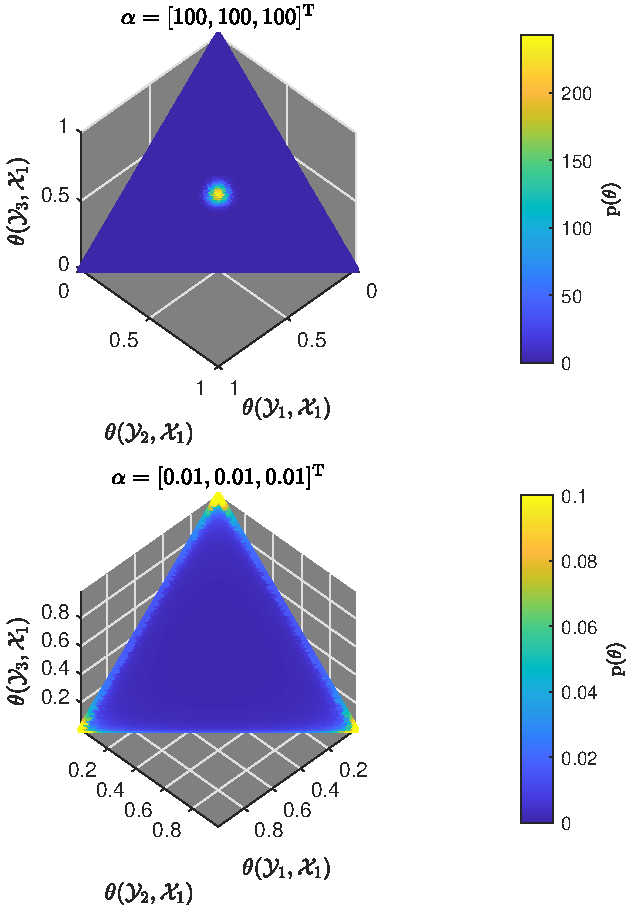
\includegraphics[width=0.8\linewidth]{P_theta.pdf}
%	\caption{Model prior PDF $\prm_{\uptheta}$ for different localizations $\alpha_0$}
%	\label{fig:P_theta}
%\end{figure}











\subsection{Bayesian Predictive Distribution}

As shown in Equation \eqref{eq:f_opt_xD}, the decision selected by the optimally designed function depends on the predictive distribution of the unobserved $\yrm$ conditioned on all observable random elements. The training data $\Drm$ is represented using the empirical sufficient statistic and $\Prm_{\yrm | \xrm,\uppsi}$ is used. Observe that $\Prm_{\yrm | \xrm,\uptheta} \equiv \upthetac(\xrm)$ and thus that $\Prm_{\yrm | \xrm,\uppsi} = \Erm_{\uptheta | \xrm,\uppsi}\big[ \Prm_{\yrm | \xrm,\uptheta} \big] \equiv \mu_{\upthetac(\xrm) | \xrm,\uppsi}$; the Bayesian predictive PMF is the posterior mean \cite{murphy} of the true predictive PMF.

Due to the independence of the conditional models $\upthetac(\xrm)$ from one another and from the marginal model, it can be shown that $\prm_{\upthetac(\xrm) | \uppsi, \xrm} \equiv \prm_{\upthetac(\xrm) | \uppsim(\xrm),\uppsic(\xrm)} \sim \Prm_{\uppsic(\xrm) | \uppsim(\xrm), \upthetac(\xrm)} \prm_{\upthetac(\xrm)}$. Since the Empirical PMF of $\uppsic(\xrm)$ has exponential form, the Dirichlet PDF $\prm_{\upthetac(\xrm)}$ is a conjugate prior \cite{theodoridis-ML}; thus, the model posterior PDF given the training data is distributed as 
\begin{IEEEeqnarray}{L}
\uptheta(\xrm) | \uppsim(\xrm),\uppsic(\xrm) \\
\quad \sim \Dir\Big( \alpha_0 \alpham(\xrm) + N \psim(\xrm), \mu_{\upthetac(\xrm) | \uppsim(\xrm), \uppsic(\xrm)} \Big) \nonumber \;,
\end{IEEEeqnarray}
Dirichlet with mean function
\begin{IEEEeqnarray}{rCl}
\mu_{\upthetac(\xrm) | \uppsim(\xrm), \uppsic(\xrm)} & = & \left( 1 + \frac{N \uppsim(\xrm)}{\alpha_0 \alpham(\xrm)} \right)^{-1} \alphac(\xrm) \nonumber \\
&& \quad + \left( 1 + \frac{\alpha_0 \alpham(\xrm)}{N \uppsim(\xrm)} \right)^{-1} \uppsic(\xrm) \nonumber \\
& \equiv & \Prm_{\yrm | \xrm,\uppsi} \;.
\end{IEEEeqnarray}
%\begin{IEEEeqnarray}{rCl}
%\mu_{\upthetac(\xrm) | \uppsim(\xrm), \uppsic(\xrm)} & = & \left(\frac{\alpha_0 \alpham(\xrm)}{\alpha_0 \alpham(\xrm) + N \uppsim(\xrm)}\right) \alphac(\xrm) \nonumber \\
%&& \quad + \left(\frac{N \uppsim(\xrm)}{\alpha_0 \alpham(\xrm) + N \uppsim(\xrm)}\right) \uppsic(\xrm) \nonumber \\
%& \equiv & \Prm_{\yrm | \xrm,\uppsi} \;.
%\end{IEEEeqnarray}
Note that as $\frac{N \uppsim(x)}{\alpha_0 \alpham(x)} \to 0$, the posterior mean tends to $\alphac(x)$, reflecting confidence in the prior mean. Conversely, as $\frac{N \uppsim(x)}{\alpha_0 \alpham(x)} \to \infty$, the Dirichlet posterior localization increases and the mean function tends to $\uppsic(\xrm)$. Consequently, $\prm_{\upthetac(x) | \uppsim(x),\uppsic(x)} \to \delta\big( \cdot - \uppsic(x) \big)$ and the model is positively identified - this is a consequence of the full support of the Dirichlet distribution. The adaptation of the posterior is demonstrated in Figure \ref{fig:P_theta_post_tilde}.
\begin{figure}
	\centering
	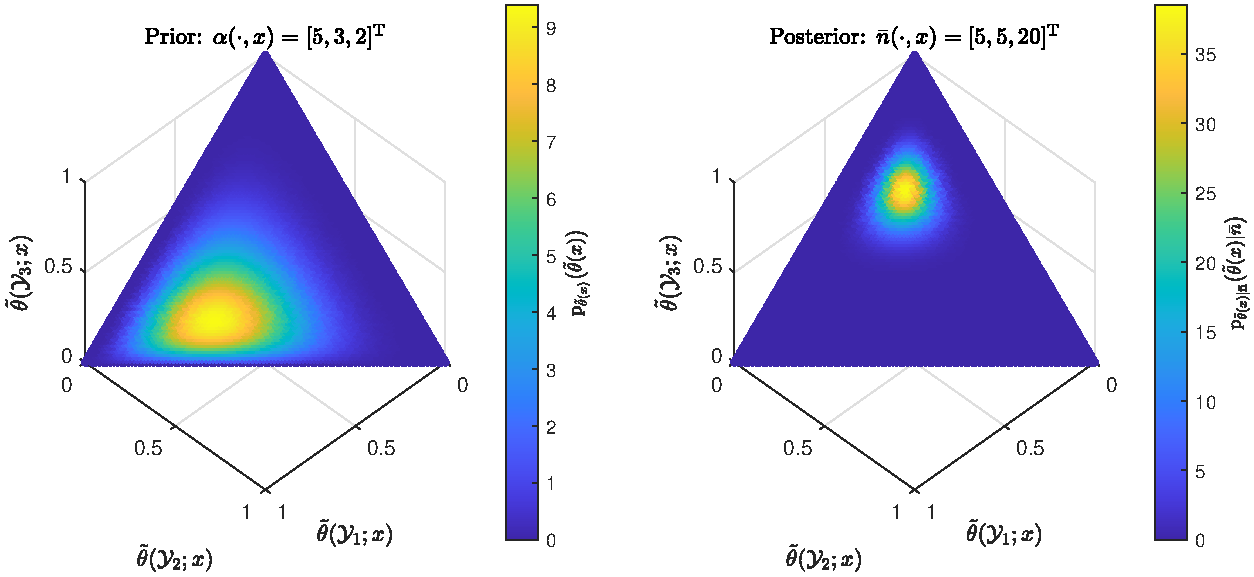
\includegraphics[width=1\linewidth]{P_theta_post_tilde_hrz.pdf}
	\caption{Model PDF, prior and posterior}
	\label{fig:P_theta_post_tilde}
\end{figure}


%The last representation views the distribution as a convex combination of two conditional distributions. The first distribution $\Prm_{\yrm | \xrm}(y | x) = \alpha(y,x) / \alpha'(x)$ is independent of the training data and based on the prior knowledge implied via the model PDF parameter; the second distribution is the conditional empirical PMF and depends solely on $\Drm$. For both, only those values $\alpha$ and $\Drm$ corresponding to the observed value of $\xrm$ influence the distribution. 
%
%The weighting factors are dependent on these values as well. For $N'(x;D) = 0$ or as $\alpha_0 \to \infty$, the PMF tends toward the conditional distribution $\Prm_{\yrm|\xrm}$, which only depends on the model parameter $\alpha$. As the number of training examples increases or as $\alpha_0 \to 0$, $\Prm_{\yrm | \xrm,\Drm}$ tends towards the empirical conditional distribution. 









\section{Regression and the Squared-Error Loss}



\subsection{Optimal Estimate: Bayesian Posterior Mean}

To find the optimal Bayesian estimator, the Bayesian predictive distribution is substituted into \eqref{eq:f_opt_xD} and the posterior mean in terms of the empirical statistic is
\begin{IEEEeqnarray}{rCl} \label{eq:f_opt_SE}
f^*(\xrm;\uppsi) & \equiv & \left( 1 + \frac{N \uppsim(\xrm)}{\alpha_0 \alpham(\xrm)} \right)^{-1} \sum_{y \in \Ycal} \alphac(y;\xrm) \ y \\
&& \quad + \left( 1 + \frac{\alpha_0 \alpham(\xrm)}{N \uppsim(\xrm)} \right)^{-1} \sum_{y \in \Ycal} \uppsic(y;\xrm) \ y \nonumber
\end{IEEEeqnarray}
%\begin{IEEEeqnarray}{rCl} \label{eq:f_opt_SE}
%f^*(\xrm;\uppsi) & \equiv & \left(\frac{\alpha_0 \alpham(\xrm)}{\alpha_0 \alpham(\xrm) + N \uppsim(\xrm)}\right) \sum_{y \in \Ycal} \alphac(y;\xrm) \ y \\
%&& \quad + \left(\frac{N \uppsim(\xrm)}{\alpha_0 \alpham(\xrm) + N \uppsim(\xrm)}\right) \sum_{y \in \Ycal} \uppsic(y;\xrm) \ y \nonumber
%\end{IEEEeqnarray}
The optimal estimate is a convex combination of first moments from two distributions - the prior mean of the conditional model, $\Prm_{\yrm | \xrm} = \mu_{\upthetac(\xrm)} = \alphac(\xrm)$, and the conditional empirical PMF. Note that expressed in terms of the training data, the second expectation is equivalent to $\frac{\sum_{n=1}^N \Yrm_n \delta[x,\Xrm_n]}{\sum_{n=1}^N \delta[x,\Xrm_n]}$.

The weighting factors are inherited from $\Prm_{\yrm | \xrm,\uppsi}$; thus, stronger prior information (larger $\alpha_0 \alpham(x)$) provides more weight to the data-independent estimate $\mu_{\yrm|\xrm}$ and higher data volume $N \uppsim(x)$ puts emphasis on the empirical mean.





\subsection{Squared-Error Risk}

Substituting the Bayesian estimator \eqref{eq:f_opt_SE} into \eqref{eq:risk_cond} and using the empirical statistic transform, the excess squared-error risk is 
\begin{IEEEeqnarray}{rCl} \label{eq:risk_cond_SE_dir_ex}
\Rcal_{\Theta, \mathrm{ex}}(f^* ; \uptheta) & = & \Erm_{\xrm,\uppsi | \uptheta} \Big[ \big( \mu_{\yrm | \xrm,\uppsi} - \mu_{\yrm | \xrm,\uptheta} \big)^2 \Big] \\
& = & \Erm_{\xrm | \upthetam}\Big[ \Sigma_{\yrm | \xrm,\upthetac} \lambda_{\text{Var}}(\xrm)  \nonumber \\
&& \quad + \left( \mu_{\yrm | \xrm} - \mu_{\yrm | \xrm,\upthetac} \right)^2 \lambda_{\text{Bias}}(\xrm) \Big] \nonumber \;,
\end{IEEEeqnarray}
a conditional expectation of two functions, where
\begin{IEEEeqnarray}{rCl}
\lambda_{\text{Var}}(x) & = & \Erm_{\uppsim(x) | \upthetam(x)}\left[ \frac{N \uppsim(x)}{\big( \alpha_0 \alpham(x) + N \uppsim(x) \big)^2} \right]
\end{IEEEeqnarray}
and
\begin{IEEEeqnarray}{rCl}
\lambda_{\text{Bias}}(x) & = & \Erm_{\uppsim(x) | \upthetam(x)}\left[ \left(\frac{\alpha_0 \alpham(x)}{\alpha_0 \alpham(x) + N \uppsim(x)}\right)^2 \right] \;.
\end{IEEEeqnarray}

The first function depends on $\Sigma_{\yrm | \xrm,\upthetac}$ and measures the estimator variance in excess of the clairvoyant squared-error. The second function is dependent on the squared bias between the clairvoyant estimate $\mu_{\yrm | \xrm,\upthetac}$ and the data-independent estimate $\mu_{\yrm | \xrm}$. 

These two second-order terms (of $y$) are scaled by factors dependent on the conditional prior localizations $\alpha_0 \alpham(x)$ and on $\upthetam(x)$ and $N$ via conditional expectations with respect to $\uppsim(x)$. By the aggregation property of Empirical distributions, $N \uppsim(x) | \upthetam(x) \sim \Bi \big(N,\upthetam(x)\big)$ is Binomially distributed. Closed-forms have not been found for the function expectations of binomial random variables above.





\subsubsection{Trends}

It is instructional to consider the trends of the squared-error risk \eqref{eq:risk_cond_SE_dir_ex} with training data volume $N$ and with Dirichlet prior parameterization. 

First consider how the excess risk depends on $N$. As $N$ tends to infinity, the distributions $\Prm_{\uppsim(x) | \upthetam(x)}$ concentrate such that $\uppsim(x) \approx \thetam(x)$; thus, the weights $\lambda_{\text{Var}}(x)$ and $\lambda_{\text{Bias}}(x)$ both tend to zero and $\Rcal_{\Theta, \mathrm{ex}}(f^* ; \uptheta) \to 0$. This desirable result is a consequence of the full support of the Dirichlet prior, ensuring that the model posterior concentrates at the empirical PMF.

An interesting point regarding the dependency of the excess risk on $N$ is that there may be a local maximum. To demonstrate, consider the case of $|\Xcal| = 1$; treating $N$ as a real number, there would be a maximum at 
\begin{equation}
N \approx \alpha_0 \left( 1 - 2 \alpha_0 \frac{\left( \mu_{\yrm | \xrm} - \mu_{\yrm | \xrm,\upthetac} \right)^2}{\Sigma_{\yrm | \xrm,\upthetac}} \right) \;.
\end{equation}
If the prior estimate $\mu_{\yrm | \xrm}$ has low bias and yet the prior confidence $\alpha_0$ is small, a local maximum may occur and additional training data may (temporarily) compromise the estimator performance. Figure \ref{fig:Risk_cond_SE_Dir_N_leg_a0_unbiased} exemplifies the excess conditional squared-error as a function of $N$ for such estimators with varying localization $\alpha_0$. 
\begin{figure}
	\centering
	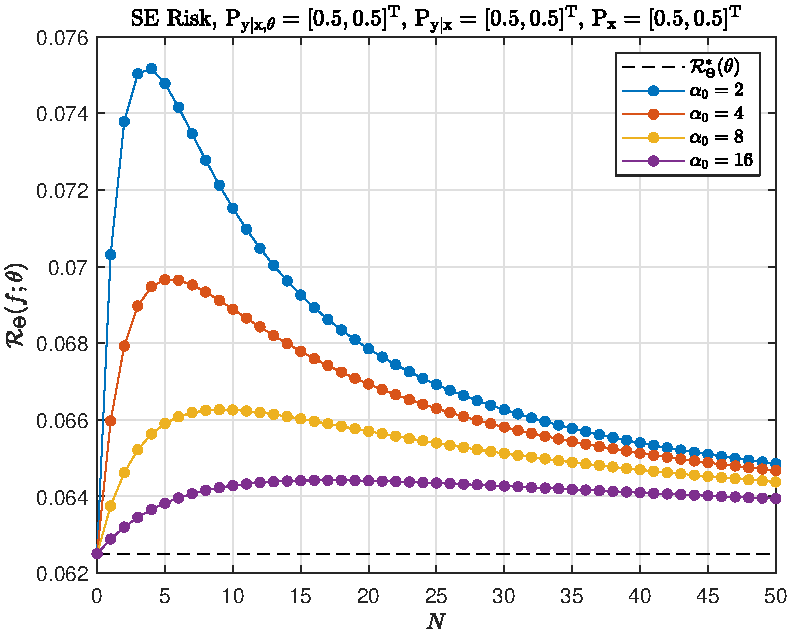
\includegraphics[width=0.9\linewidth]{Risk_cond_SE_Dir_N_leg_a0_unbiased.pdf}
	\caption{Squared-Error Risk for unbiased Dirichlet estimators}
	\label{fig:Risk_cond_SE_Dir_N_leg_a0_unbiased}
\end{figure}



Next consider the effects of the conditional prior localizations $\alpha'(x) \equiv \alpha_0 \alpham(x)$, which control a bias/variance risk trade-off. For maximal localization $\alpha'(x) \to \infty$, $\lambda_{\text{Bias}}(x) \to 1$ and $\lambda_{\text{Var}}(x) \to 0$. This is intuitive given that the estimator tends toward the data-independent solution. Conversely, for $\alpha'(x) \to 0$, $\lambda_{\text{Bias}}(x) \to \big( 1 - \upthetam(\xrm) \big)^N$ and $\lambda_{\text{Var}}(x) \to \Erm_{\uppsim(x) | \upthetam(x)}\left[ \big( N \uppsim(x) \big)^{-1} \right]$. Note that the variance weight is equivalent to the first inverse moment of a positive binomial random variable \cite{stephan}. 


Of primary interest are the values $\alpha'(x)$ that minimize the excess squared-error for given prior conditional distributions $\alphac(x)$. Calculating the first derivative, it can be shown that (for $N > 0$ and $\thetam(x) > 0$) only one stationary point exists at 
\begin{equation} \label{eq:alpha_x_min_Rex}
\alpha'(\xrm) = \frac{\Sigma_{\yrm | \xrm,\upthetac}}{\left( \mu_{\yrm | \xrm} - \mu_{\yrm | \xrm,\upthetac} \right)^2} \;.
\end{equation}
Evaluation of the second derivative confirms the local maximum and comparison of the local risk value to the $\alpha'(x) \to 0$ and $\alpha'(x) \to \infty$ limits confirms the global minimum.


Note that the minimizing concentration values $\alpha'(x)$ are inversely proportional to the squared-bias of the prior conditional mean. This is sensible; the better the match between the true and prior predictive distributions, the more confidence should be expressed. Also, low concentrations are preferable when the conditional model has low variance; these models can be accurately identified by learners that emphasize the empirical mean, even with limited training data. These trends are demonstrated by Figure \ref{fig:Risk_cond_SE_Dir_a0_leg_N_biased}.

\begin{figure}
	\centering
	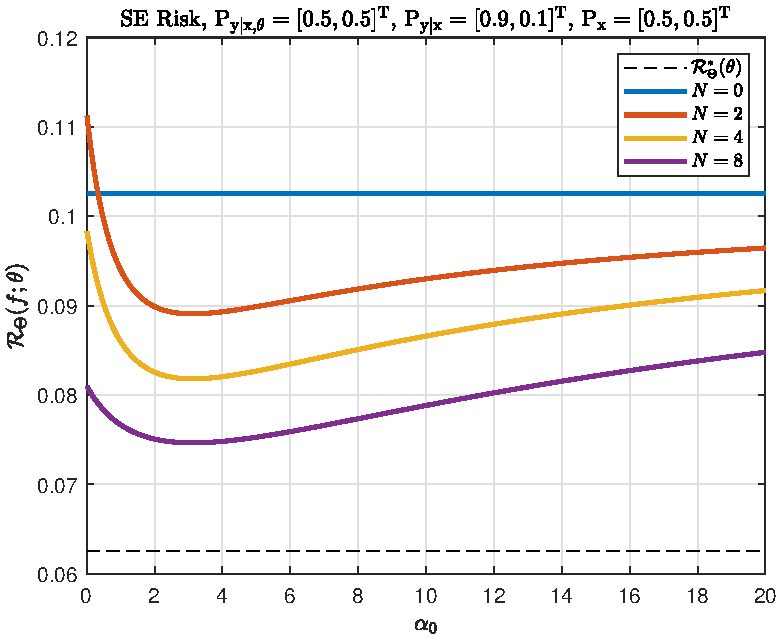
\includegraphics[width=0.9\linewidth]{Risk_cond_SE_Dir_a0_leg_N_biased.pdf}
	\caption{Conditional SE Risk versus $\alpha_0$, biased Dirichlet estimator using varying training set volumes}
	\label{fig:Risk_cond_SE_Dir_a0_leg_N_biased}
\end{figure}







\section{Conclusions}

This paper has assumed a Dirichlet prior for Bayesian learning and applied the resultant predictive distribution to squared-error regression. Closed-forms have been provided for the optimal estimator and the achieved risk. Analysis and graphical examples highlight risk trends as a function of training data volume and the Dirichlet prior localization, demonstating a bias/variance risk trade-off.

Future work will generalize these concepts for data drawn from Euclidean spaces using the continuous Dirichlet process. Additionally, these estimators will be compared to classical methods such as generalized linear regression. The inherent adaptability due to the full prior support will highlight the utility of these Bayesian estimators for a wide range of regression problems; however, for data-limited problems, the ``prior knowledge'' implied by classical methods can yield superior performance when the data model is well understood.











\bibliographystyle{IEEEtran}
\bibliography{{../References/phd_bib}}


\end{document}


























